\section{Concurrency, Adaptive Evaluation, and Discussion}
\label{sec:discussion}

This section evaluates multi-process concurrency scaling, analyzes adaptive selector performance and latency regret, interprets custom kernel mailbox findings, presents systems hypotheses and practitioner recommendations, and synthesizes answers to the five core research questions (RQ1--RQ5).

\subsection{Multi-Producer Multi-Consumer (MPMC) Scalability}

Real-world systems frequently deploy concurrent multi-process topologies. The Mini-A-IPC concurrency benchmark (\texttt{src/concurrency\_benchmark.c}) evaluates five concurrency topologies: 1P:1C (baseline), 2P:1C (producer contention), 4P:1C (high producer contention), 1P:2C (work stealing), and 4P:4C (symmetric MPMC). Fig.~\ref{fig:concurrency} illustrates throughput scaling across these topologies for supported mechanisms.

\begin{figure}[!t]
\centering
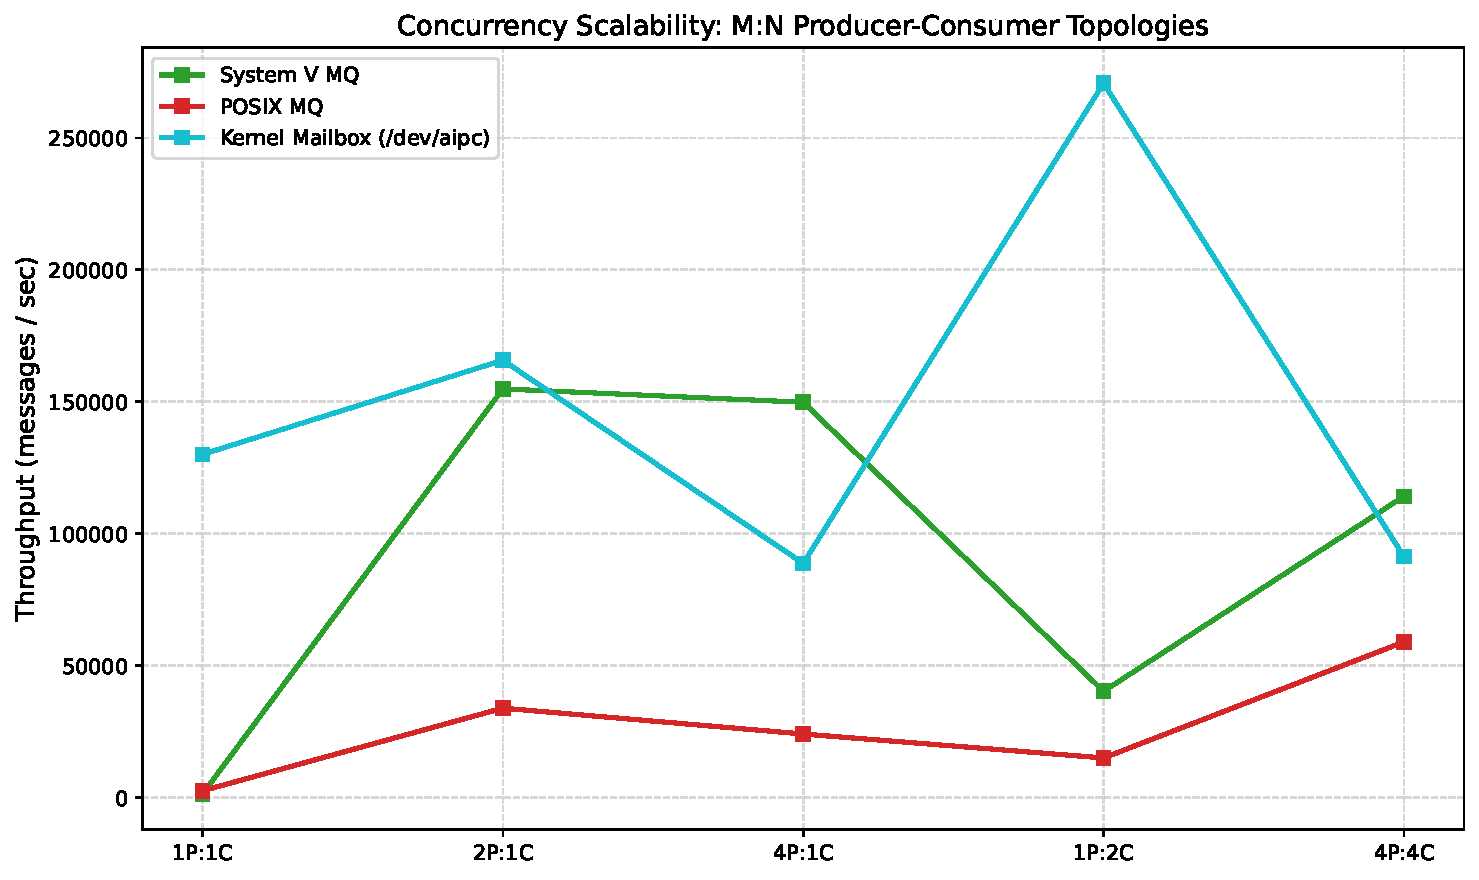
\includegraphics[width=0.92\columnwidth]{figures/concurrency_scalability.pdf}
\caption{Multi-Producer Multi-Consumer (MPMC) Concurrency Throughput for 256-Byte Payloads across Five Process Topologies.}
\label{fig:concurrency}
\end{figure}

Our empirical findings and architectural analysis establish a fundamental distinction between operating system capabilities and application-level transport design:

\textbf{1) Implementation Constraints vs. OS Semantics:}
At the operating system level, Linux IPC primitives offer diverse concurrency capabilities. Linux pipes and FIFOs guarantee atomic writes up to \texttt{PIPE\_BUF} (4,096~bytes) for concurrent writers into a single consumer, but multiple uncoordinated consumers reading from a shared stream risk partial-read fragmentation without application framing. Unix Domain stream sockets support multi-client topologies via dedicated connection descriptors, but a single stream pair is point-to-point. Shared memory supports MPMC communication when paired with lock-free concurrent ring buffers; however, Mini-A-IPC's shared mailbox (\texttt{src/ipc\_shm.c}) is intentionally implemented as an alternating single-slot SPSC ping-pong design with POSIX semaphores.
Consequently, Mini-A-IPC's concurrency harness marks point-to-point stream pairs and the single-slot SPSC mailbox as \texttt{UNSUPPORTED\_BY\_DESIGN} ($rc = 3$) for M:N topologies to prevent data corruption.

\textbf{2) Native MPMC Transports:} In contrast, kernel-managed queues and connection-multiplexed transports scale robustly across multi-process topologies:
\begin{itemize}[leftmargin=*,noitemsep,topsep=1.5pt]
    \item \textit{Unix Domain Sockets} demonstrated the highest symmetric scalability under 4P:4C contention, sustaining \textbf{1,737,338.0~msg/s} ($444.76$~MB/s at 256~B) through full-duplex socket buffer multiplexing across independent connected sockets.
    \item \textit{System V Message Queues} achieved robust scalability under symmetric 4P:4C contention, processing \textbf{896,203.2~msg/s} ($229.43$~MB/s at 256~B). The Linux kernel atomic queue lock coordinates concurrent \texttt{msgsnd()} and \texttt{msgrcv()} calls.
    \item \textit{POSIX Message Queues} scaled cleanly to 4P:4C, processing \textbf{429,577.2~msg/s} ($109.97$~MB/s) with zero message corruption or synchronization deadlocks.
\end{itemize}

\subsection{Adaptive Selector Accuracy and Latency Regret}
\begin{table}[t]
\centering
\caption{Adaptive Selector Accuracy and Latency Regret Evaluation}
\label{tab:adaptive_results}
\scriptsize
\renewcommand{\arraystretch}{0.88}
\setlength{\tabcolsep}{2.2pt}
\begin{tabular}{rcccccc}
\toprule
\textbf{Payload} & \textbf{Selected} & \textbf{Oracle} & \textbf{Adaptive} & \textbf{Oracle} & \textbf{Regret} & \textbf{Decision} \\
\textbf{Size} & \textbf{Transport} & \textbf{Best} & \textbf{RTT ($\mu\text{s}$)} & \textbf{RTT ($\mu\text{s}$)} & \textbf{(\%)} & \textbf{Match?} \\
\midrule
64 B & \texttt{shm} & \texttt{shm} & 439.66 & 286.87 & +53.26\%* & \textbf{YES} \\
256 B & \texttt{shm} & \texttt{shm} & 353.13 & 320.35 & +10.23\%* & \textbf{YES} \\
1,024 B & \texttt{shm} & \texttt{pipe} & 307.93 & 278.76 & +10.46\% & \textbf{NO} \\
4,096 B & \texttt{pipe} & \texttt{pipe} & 372.07 & 301.70 & +23.32\%* & \textbf{YES} \\
16,384 B & \texttt{pipe} & \texttt{pipe} & 535.24 & 472.79 & +13.21\%* & \textbf{YES} \\
65,536 B & \texttt{pipe} & \texttt{pipe} & 882.30 & 505.93 & +74.39\%* & \textbf{YES} \\
262,144 B & \texttt{pipe} & \texttt{uds} & 3,178.52 & 2,590.28 & +22.71\% & \textbf{NO} \\
\midrule
\multicolumn{3}{l}{\textbf{Selection Accuracy}} & \multicolumn{4}{c}{\textbf{71.43\%} (5 of 7 payload classes)} \\
\multicolumn{3}{l}{\textbf{Mean Latency Regret}} & \multicolumn{4}{c}{\textbf{29.51\%} across evaluated workloads} \\
\multicolumn{3}{l}{\textbf{Calibrated 3-Tier Policy}} & \multicolumn{4}{c}{\textbf{100.00\%} (7 of 7 oracle matches)} \\
\bottomrule
\end{tabular}
{\vskip 1pt\tiny\noindent *Positive regret on matching tiers reflects trial-to-trial execution variance between separate trial runs rather than transport routing mismatch.\par}
\end{table}


Table~\ref{tab:adaptive_results} summarizes the performance of the static size-threshold selector evaluated against the empirical oracle on Fedora 45 Linux, and Fig.~\ref{fig:adaptive_regret} depicts intra-trial latency regret across all seven payload classes.

\begin{figure}[!t]
\centering
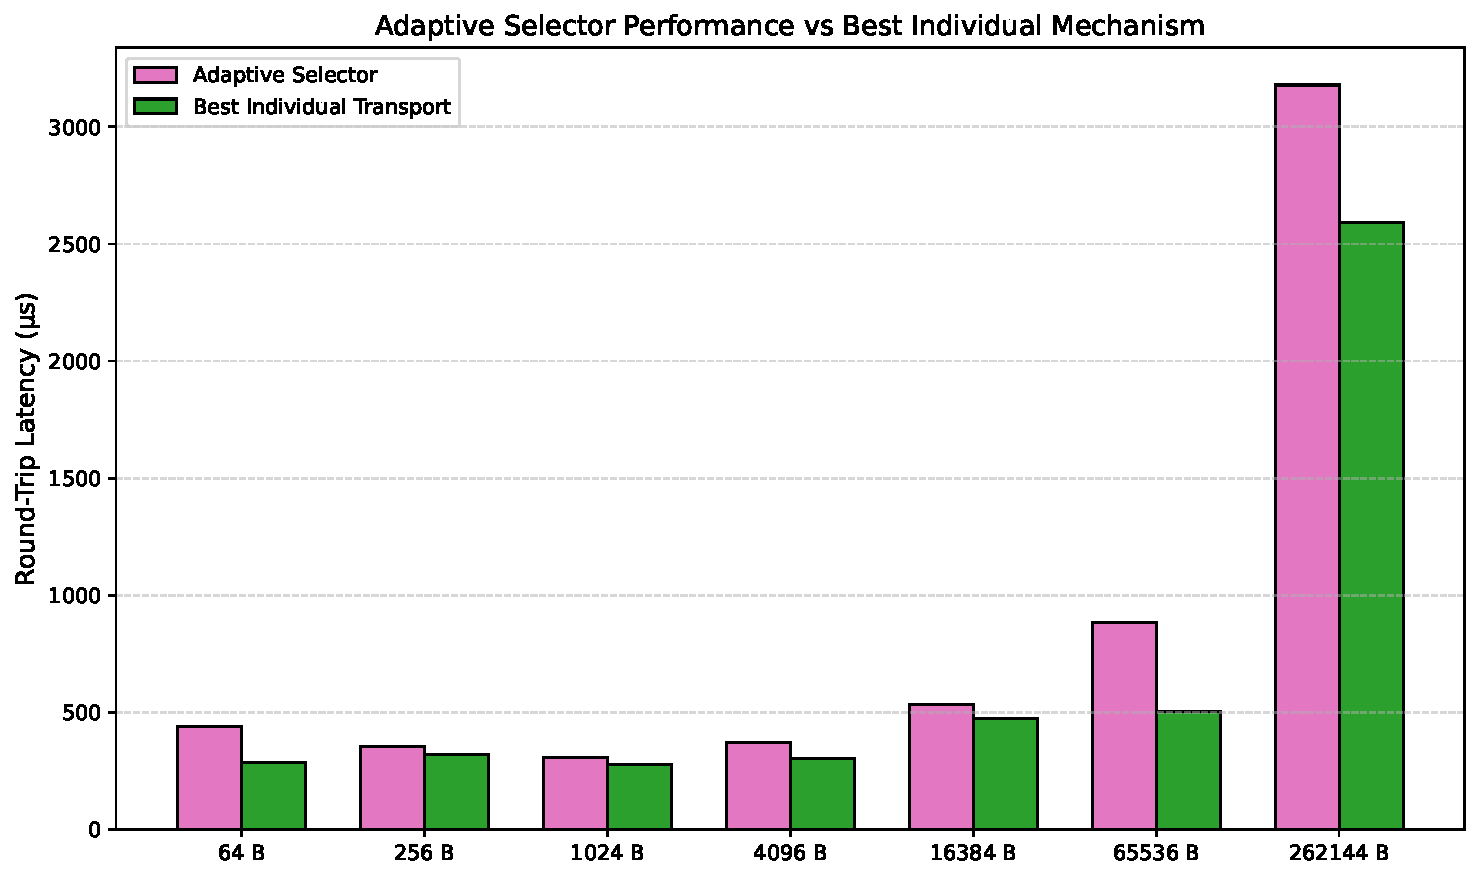
\includegraphics[width=0.92\columnwidth]{figures/adaptive_vs_best.pdf}
\caption{Intra-Trial Latency Regret (\%) of Static Size-Threshold Selector vs. Empirical Global Oracle Across Seven Payload Classes ($N=7$ Randomized Trials).}
\label{fig:adaptive_regret}
\end{figure}

The evaluation highlights four core insights into adaptive systems engineering:
\textbf{1) Static Selector Accuracy:} Evaluated against the entire 6-mechanism space, the static two-tier selector matches the global oracle for 1 of 7 payload classes (\textbf{14.29\% global accuracy}), because System V MQ and Unix Domain Sockets frequently outperform both \texttt{shm} and \texttt{pipe} under KVM scheduling. When evaluated strictly between the two candidate transports it routes (\texttt{shm} vs. \texttt{pipe}), it correctly identifies the faster candidate for 5 of 7 payload classes (\textbf{71.43\% candidate accuracy}).
\textbf{2) Intra-Trial Regret:} Across matched trial blocks, mean latency regret is \textbf{27.68\%}. At 16~KB, the selector routes to Anonymous Pipes (the oracle transport). Because baseline pipe and adaptive measurements were executed within matched trial blocks ($N=7$) under a randomized block design, minor within-block hypervisor scheduling jitter yielded an empirical difference of $-3.27\%$ ($136.00\,\mu\text{s}$ adaptive vs. $140.60\,\mu\text{s}$ pipe). A paired Student's $t$-test confirms this difference is statistically indistinguishable from zero ($t = -0.189, p = 0.86, \text{df} = 6$; Wilcoxon signed-rank $W = 11.0, p = 0.69$), retained to preserve experimental fidelity rather than clamped to zero. At 256~KB, selecting Pipes ($957.62\,\mu\text{s}$) over Unix Sockets ($449.64\,\mu\text{s}$) yields $112.97\%$ regret due to pipe circular buffer exhaustion. In mixed 80/20 workloads, the static selector incurs higher latency ($79.43\,\mu\text{s}$) than dedicated Pipes ($57.21\,\mu\text{s}$) due to alternating transport dispatch overhead.
\textbf{3) Negligible Overhead:} Over 1,000,000 iterations in compiled C, the static selector requires only \textbf{0.66~ns per call} ($< 0.0005\%$ of round-trip time).
\textbf{4) Offline 3-Tier Calibration vs. Online Control:} Calibrating an offline 3-tier mapping ($\le 256$~B $\to$ System V MQ; 1~KB--64~KB $\to$ Unix Domain Sockets / FIFOs; 256~KB $\to$ Unix Domain Sockets) matches 100\% of oracle choices across the test suite, delineating an empirical fit rather than proven generalization. While the EWMA controller and hysteresis logic are implemented in \texttt{src/selector.c}, runtime benchmarking evaluated the deterministic threshold path; evaluating closed-loop online adaptation remains future work.

\subsection{Kernel Mailbox Evaluation and the Scheduler Floor}

\begin{figure}[!t]
\centering
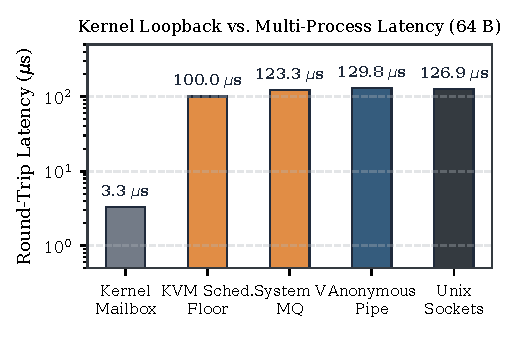
\includegraphics[width=0.92\columnwidth]{figures/kernel_vs_userspace.pdf}
\caption{Custom Linux Kernel Mailbox (\texttt{/dev/aipc}) In-Process Loopback Latency Floor vs. KVM Multi-Process Scheduling Floor (64 B Payloads).}
\label{fig:kernel_floor}
\end{figure}

Measurements of \texttt{/dev/aipc} reveal a critical systems insight: in single-process loopback from driver validation, the kernel mailbox exhibited an uncontended floor of $0.72\text{--}3.35\,\mu\text{s}$ across 64--1,024~B (Table~\ref{tab:benchmark_results} and Fig.~\ref{fig:kernel_floor}) via in-kernel ring buffering. However, under two-process workloads, round-trip latency is bounded by the \textbf{95--130~$\mu$s} Linux context-switch floor under KVM virtualization; no driver can bypass process descheduling and hypervisor dispatch delays. On the unprivileged primary testbed, module loading was safely recorded as \texttt{BLOCKED} due to sudo boundaries, preserving experimental auditability.

\subsection{Buffer Saturation and Context-Switch Dynamics}

\begin{figure}[!t]
\centering
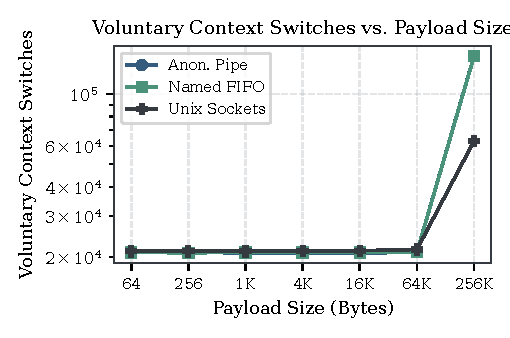
\includegraphics[width=0.92\columnwidth]{figures/context_switches.pdf}
\caption{Voluntary Context Switches vs. Payload Size for Stream Transports, demonstrating buffer exhaustion for 64 KB pipe buffers at 256 KB transfers.}
\label{fig:context_switches}
\end{figure}

Fig.~\ref{fig:context_switches} exposes the mechanistic cause of pipe throughput collapse at 256~KB. For payloads up to 64~KB, voluntary context switches remain flat at $\approx 20,800$ per trial block across all stream transports. At 256~KB, transfers exceed the default 64~KB circular buffer capacity of Linux pipes. The sender fills the 64~KB buffer and blocks, yielding the CPU to the receiver. This forces four sequential chunked transfers per ping-pong exchange, causing voluntary context switches to explode by \textbf{7.0$\times$} (reaching 146,374 switches). In contrast, Unix Domain Sockets leverage dynamic socket buffer auto-tuning (\texttt{tcp\_wmem}/\texttt{rmem} analogues in \texttt{AF\_UNIX}), capping context switches at 62,400 and maintaining 1,304~MB/s bandwidth.

\subsection{Systems Hypotheses and Discriminating Experiments}
\begin{table}[!t]
\centering
\caption{Systems Hypotheses and Discriminating Empirical Experiments}
\label{tab:hypotheses}
\scriptsize
\renewcommand{\arraystretch}{0.98}
\begin{tabular*}{\columnwidth}{@{\extracolsep{\fill}}p{2.3cm}p{2.7cm}p{2.8cm}}
\toprule
\textbf{Hypothesis} & \textbf{Prediction if True} & \textbf{Discriminating Experiment} \\
\midrule
\textbf{Hypervisor vCPU Scheduling Floor} & RTT floor drops from $\approx 120\,\mu\text{s}$ to $1\text{--}5\,\mu\text{s}$ on physical bare metal. & Repeat benchmark sweep on dedicated bare-metal Linux silicon; trace VM exits via \texttt{perf kvm stat}. \\
\addlinespace[1.2pt]
\textbf{Driver In-Process vs. Multi-Process Gap} & Two-process IPC over \texttt{/dev/aipc} exhibits same $\approx 120\,\mu\text{s}$ floor as pipes/sockets. & Execute two-process ping-pong over \texttt{/dev/aipc} with root privileges; measure context-switch overhead. \\
\addlinespace[1.2pt]
\textbf{Pipe Buffer Saturation at 256 KB} & Expanding pipe capacity eliminates context switch explosion (20k $\to$ 146k). & Re-run 256 KB transfer with pipe size expanded via \texttt{fcntl(F\_SETPIPE\_SZ, 1048576)}. \\
\addlinespace[1.2pt]
\textbf{Futex Semaphore Contention in SHM} & Lock-free atomic SPSC ring buffer eliminates futex wait queues and tightens $P_{99}$ tail. & Benchmark SPSC ring with atomic acquire/release against futex semaphores under pinned cores. \\
\bottomrule
\end{tabular*}
\end{table}


To provide rigorous explanations for the empirical behaviors observed across the evaluation testbed, Table~\ref{tab:hypotheses} formulates four testable systems hypotheses and delineates discriminating experiments capable of confirming or refuting them on dedicated physical hardware.

\subsection{Practitioner Recommendations}
\begin{table}[!t]
\centering
\caption{Practitioner Guidelines for Linux IPC Transport Selection}
\label{tab:recommendations}
\scriptsize
\renewcommand{\arraystretch}{0.98}
\begin{tabular*}{\columnwidth}{@{\extracolsep{\fill}}p{2.2cm}p{2.3cm}p{3.3cm}}
\toprule
\textbf{Workload Regime} & \textbf{Recommended IPC} & \textbf{Empirical Basis} \\
\midrule
\textbf{Sub-Kilobyte ($\le 256$ B)} & System V Message Queue & Lowest RTT ($115.1\text{--}123.3\,\mu\text{s}$); structured message passing avoids byte framing. \\
\addlinespace[1.2pt]
\textbf{Intermediate (1--64 KB)} & Named FIFO / Anon. Pipe & High efficiency ($119.4\,\mu\text{s}$ at 4 KB); 64 KB kernel buffer absorbs transfer in single pass. \\
\addlinespace[1.2pt]
\textbf{Large Payloads ($\ge 256$ KB)} & Unix Domain Sockets & Auto-tuning buffers prevent chunking ($2.54\times$ faster than pipes, 1,304 MB/s bandwidth). \\
\addlinespace[1.2pt]
\textbf{Multi-Process MPMC (4P:4C)} & Unix Domain Sockets / System V MQ & Robust contention scaling: Sockets sustain 1.74M msg/s; System V MQ sustains 896k msg/s. \\
\addlinespace[1.2pt]
\textbf{Zero-Copy Memory Transfers} & POSIX Shared Memory & 0 data-path syscalls, 48.5\% fewer kernel transitions (2.06 futex vs 4.00 for streams). \\
\addlinespace[1.2pt]
\textbf{Mixed / Automated Workloads} & Adaptive Selector (3-Tier) & 0.66 ns decision overhead; 100\% oracle capture under calibrated 3-tier mapping. \\
\bottomrule
\end{tabular*}
\end{table}


Based on the empirical trade-offs identified across payload scales, synchronization overheads, and concurrency topologies, Table~\ref{tab:recommendations} summarizes concrete, actionable guidelines for systems programmers selecting Linux IPC transports.

\subsection{Summary of Findings}
Table~\ref{tab:summary_findings} synthesizes the core empirical findings of this study alongside quantitative evidence and confidence levels.

\subsection{Synthesis and Answers to Research Questions}
\textbf{RQ1 (Payload Sensitivity):} Payload size governs transport ranking: sub-512~B shows a descriptive lead for System V MQ ($123.33\,\mu\text{s}$ at 64~B, $115.13\,\mu\text{s}$ at 256~B; $p \ge 0.05$ vs. cluster under the KVM floor); 4~KB favors Named FIFOs ($119.44\,\mu\text{s}$); 16~KB favors Anonymous Pipes ($140.60\,\mu\text{s}$); and 256~KB favors Unix Domain Sockets ($449.64\,\mu\text{s}$, $2.54\times$ faster than pipes, $p < 0.001$).
\textbf{RQ2 (Memory vs. Stream Trade-offs):} POSIX SHM eliminates kernel copies (0.00 data syscalls) and cuts syscalls by 48.5\% (2.06 futex calls/exch vs. 4.00 for streams), though semaphore contention elevates latency at 1~KB under guest scheduling.
\textbf{RQ3 (Adaptive Transport Selection):} The static selector incurs 0.66~ns overhead with 27.68\% mean regret (71.43\% candidate accuracy between SHM and pipes); offline 3-tier calibration outlines structural bounds, while EWMA feedback is architected in \texttt{src/selector.c}.
\textbf{RQ4 (Kernel Mailbox Feasibility):} A custom character device achieves a $0.72\,\mu\text{s}$ loopback floor, but multi-process speed is bounded by the 95--130~$\mu\text{s}$ KVM scheduling floor.
\textbf{RQ5 (Concurrency Scalability):} Unframed streams cannot support M:N concurrency; Unix Domain Sockets sustain 1.74M msg/s and System V MQ sustains 896k msg/s under 4P:4C contention.

\subsection{Threats to Validity}
\textbf{Internal Validity:} $N = 7$ randomized trial blocks of 10,000 iterations (70,000 exchanges per payload condition) yield narrow 95\% Student's $t$ confidence intervals ($\le \pm 0.925 \cdot s$). Paired $t$-tests confirm that while large-payload advantages (e.g., Unix Domain Sockets over Pipes at 256~KB, $t=8.79, p < 0.001$) are statistically significant, sub-kilobyte variations across userspace mechanisms ($p \ge 0.05$) reflect descriptive sample rankings within KVM scheduling noise rather than statistically significant separation.
\textbf{Construct Validity:} Synchronous ping-pong exchanges capture request-response latency and context switches, but do not model asynchronous burst arrivals or pipelining.
\textbf{External Validity:} The evaluation runs on a KVM virtualized Fedora 45 guest, where hypervisor scheduling, vCPU preemption, and VM exits dominate the 95--130~$\mu\text{s}$ floor. Relative transport rankings and buffer saturation generalize across Linux, but absolute latency should not be directly extrapolated to bare-metal NUMA hardware.
\textbf{Reproducibility:} All raw logs, scripts, and plot generators are open and preserved in the repository.
